
\documentclass[twocolumn, amsmath]{revtex4}

\usepackage{graphicx}



\begin{document}


\title{PHYS 605 Lab \#9} 

\author{Morgan Daly}
\author{Evin O'Shea}
\date{\today} 


\maketitle


\section{Introduction and Theory}
\subsection{Purpose}

The goal was to build a 4-bit shift register using D flip-flops. This required application of logic concepts to understand the behavior of the D flip-flop.


\subsection{Background / Theory}

A set-reset flip-flop is made up of two NOR (``not or") gates whose output and inputs are connected as shown in figure (1).

\begin{figure}[h]
    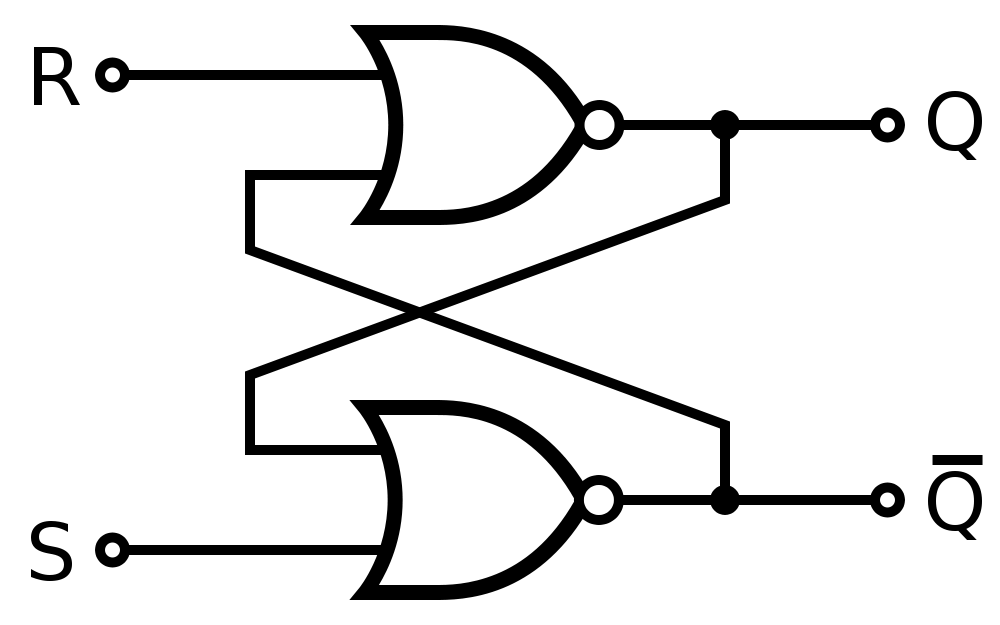
\includegraphics[scale=0.18]{setreset}  
    \caption{A set-reset flip-flop.}
\end{figure}

% could describe the logic here in depth
The output of the set-reset flip-flop is low when S=0 and R=1, and high when S=1 and R=0. When its inputs are not opposite, its behavior is undefined. The SR flip-flop's truth table is shown below.

\begin{center}
	\begin{ruledtabular}
    \begin{tabular}{ l l l}
	S & R & Q\\ \colrule
	0 & 0 & X \\
	0 & 1 & 0 \\
	1 & 0 & 1
\end{tabular}
    \end{ruledtabular}
\end{center}

A 555 timer is a device which produces timing pulses. The frequency of these pulses depend on the resistor values, $R_a$ and $R_b$, and capacitor value, $C$.

\begin{equation}
f = \frac{1.4}{C(R_a + 2R_b)}
\end{equation}

A D flip-flop, shown in figure (2), takes the data line at its D terminal, and a clock input at the CLK terminal as input. Internally, it is made up of two gated set-reset flip-flops. These gates enable the SR flip-flop only when E is high. In the D flip-flop, the clock input is what is connected to the second E, and the first takes E after it has gone through an inverter. This means that when the clock is low, the first SR flip-flop is enabled, and when the clock is high, the second SR flip-flop is enabled. 
The data line should be bits, so the D input will be either low or high. S1 takes D directly, and R1 takes D after it is inverted. This means that its output will always be 0 at one terminal and 1 at the other (as its terminals are ``Q" and ``not Q"). This means that the inputs to the second SR flip-flop will also be 0 at one terminal and 1 at the other. This is important because it ensures that the output of the SR flip-flops will be reasonable.

\begin{figure}[h]
    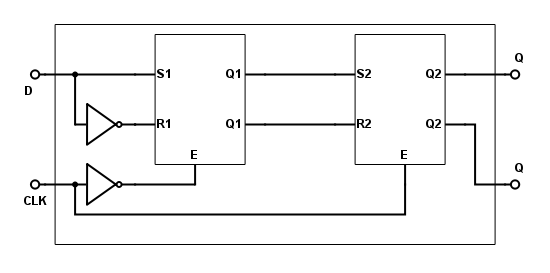
\includegraphics[scale=0.45]{dflipflop}  
    \caption{Detailed view of a D flip-flop.}
\end{figure}

\begin{center}
	\begin{ruledtabular}
    \begin{tabular}{ l l l}
	D & CLK & Q\\ \colrule
	0 & rising edge & 0 \\
	1 & rising edge & 1 \\
\end{tabular}
    \end{ruledtabular}
\end{center}

A shift resistor is a circuit that propagates bits in support of memory management. It takes data in at one terminal, and shifts one bit on each clock pulse that is input to the other terminal. It is constructed by cascading flip-flops so that the output of one flip-flop is the input of the next flip-flop. All are connected to the same clock. 

%figure 4 because adding 555 timer pic?
A 4-bit shift register is made up of four flip-flops, as shown in figure (4). 

\begin{figure}[h]
    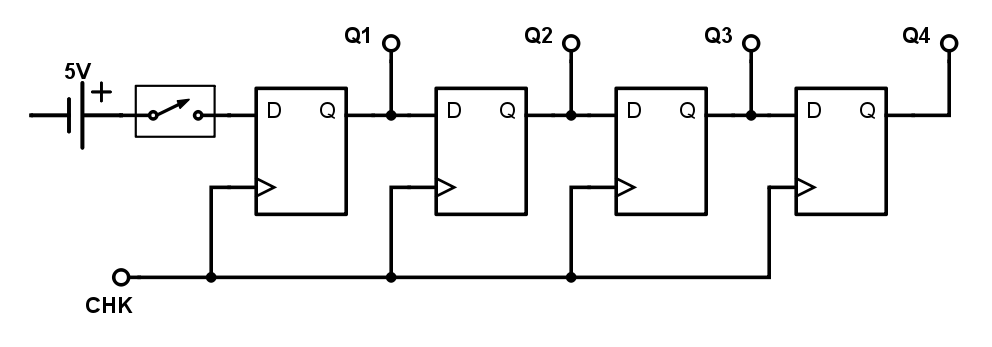
\includegraphics[scale=0.26]{bitshifter.png}  
    \caption{The shift register schematic.}
\end{figure}

This kind of shift register is known as serial-in, parallel-out (SIPO), because the bits are provided in serial through the data line D, and then are pushed through the shift register one step at a time on each clock pulse. 
This means that after four clock pulses, four bits will have been loaded: one for each output Q. The information is then available in parallel.


\section{Methodology}

\begin{enumerate}
	\item Using equation (1), select resistor and capacitor values that will create a frequency that makes the circuit behavior easy to observe.
	\item Set up 555 timer.
    \item Construct the shift registor circuit as shown in figure (2). 
    \item Connect an LED to each output Q.
    \item Using the switch to change the input to the circuit and observe the behavior of the LEDS.
\end{enumerate}


\section{Results and Analysis}
% No clue what values we used
In setting up the 555 timer, $R_a$ was chosen to be $X \Omega$,$R_b$ was chosen to be $X \Omega$, and $C$ was chosen to be XF. Using equation (1), this gave an expected frequency of XHz.

\begin{equation*}
\begin{aligned}
f_{expected} &= \frac{1.4}{C(R_a + 2R_b)}\\ &= \frac{1.4}{0.947\times 10^{-6}(2(677\times 10^3) + 35.18\times 10^3}\\ &= 1.98 Hz
\end{aligned}
\end{equation*}

This was effective, as the clock pulses were slow enough that they were easy to observe.

When the "data" was given to the circuit by flipping the switch to provide the 5V input, the LED at Q1 lit up, followed by the LED at Q2, then Q3, then Q4; when Q4 lit up all four LEDs were lit. When the switch was opened so that no voltage was provided to the input D, the LED at Q4 dimmed first, then Q3, then Q2, and finally Q1. 

This behavior was what was expected, as the bit register should push the bit forward a step on each clock pulse.



\section{Conclusion}

The shift register was built successfully. The LEDs at each output lit as the "bit" was pushed through, then turned off one at a time beginning with Q4 and ending with Q1.

\end{document}

